
%<<setup-child, include = FALSE>>=
%library(knitr)
%library(ggplot2)
%library(microbenchmark)
%set_parent("../style/preamble.Rnw")
%@

\input{../../2021/style/preamble4tex}
% dependencies: amsmath, amssymb, dsfont
% math spaces
\ifdefined\N
\renewcommand{\N}{\mathds{N}} % N, naturals
\else \newcommand{\N}{\mathds{N}} \fi
\newcommand{\Z}{\mathds{Z}} % Z, integers
\newcommand{\Q}{\mathds{Q}} % Q, rationals
\newcommand{\R}{\mathds{R}} % R, reals
\ifdefined\C
\renewcommand{\C}{\mathds{C}} % C, complex
\else \newcommand{\C}{\mathds{C}} \fi
\newcommand{\continuous}{\mathcal{C}} % C, space of continuous functions
\newcommand{\M}{\mathcal{M}} % machine numbers
\newcommand{\epsm}{\epsilon_m} % maximum error

% counting / finite sets
\newcommand{\setzo}{\{0, 1\}} % set 0, 1
\newcommand{\setmp}{\{-1, +1\}} % set -1, 1
\newcommand{\unitint}{[0, 1]} % unit interval

% basic math stuff
\newcommand{\xt}{\tilde x} % x tilde
\newcommand{\argmin}{\mathop{\mathrm{arg\,min}}} % argmin
\newcommand{\argmax}{\mathop{\mathrm{arg\,max}}} % argmax
\newcommand{\argminlim}{\argmin\limits} % argmin with limits
\newcommand{\argmaxlim}{\argmax\limits} % argmax with limits
\newcommand{\sign}{\operatorname{sign}} % sign, signum
\newcommand{\I}{\mathbb{I}} % I, indicator
\newcommand{\order}{\mathcal{O}} % O, order
\newcommand{\bigO}{\mathcal{O}} % Big-O Landau
\newcommand{\littleo}{{o}} % Little-o Landau
\newcommand{\pd}[2]{\frac{\partial{#1}}{\partial #2}} % partial derivative
\newcommand{\floorlr}[1]{\left\lfloor #1 \right\rfloor} % floor
\newcommand{\ceillr}[1]{\left\lceil #1 \right\rceil} % ceiling
\newcommand{\indep}{\perp \!\!\! \perp} % independence symbol

% sums and products
\newcommand{\sumin}{\sum\limits_{i=1}^n} % summation from i=1 to n
\newcommand{\sumim}{\sum\limits_{i=1}^m} % summation from i=1 to m
\newcommand{\sumjn}{\sum\limits_{j=1}^n} % summation from j=1 to p
\newcommand{\sumjp}{\sum\limits_{j=1}^p} % summation from j=1 to p
\newcommand{\sumik}{\sum\limits_{i=1}^k} % summation from i=1 to k
\newcommand{\sumkg}{\sum\limits_{k=1}^g} % summation from k=1 to g
\newcommand{\sumjg}{\sum\limits_{j=1}^g} % summation from j=1 to g
\newcommand{\summM}{\sum\limits_{m=1}^M} % summation from m=1 to M
\newcommand{\meanin}{\frac{1}{n} \sum\limits_{i=1}^n} % mean from i=1 to n
\newcommand{\meanim}{\frac{1}{m} \sum\limits_{i=1}^m} % mean from i=1 to n
\newcommand{\meankg}{\frac{1}{g} \sum\limits_{k=1}^g} % mean from k=1 to g
\newcommand{\meanmM}{\frac{1}{M} \sum\limits_{m=1}^M} % mean from m=1 to M
\newcommand{\prodin}{\prod\limits_{i=1}^n} % product from i=1 to n
\newcommand{\prodkg}{\prod\limits_{k=1}^g} % product from k=1 to g
\newcommand{\prodjp}{\prod\limits_{j=1}^p} % product from j=1 to p

% linear algebra
\newcommand{\one}{\bm{1}} % 1, unitvector
\newcommand{\zero}{\mathbf{0}} % 0-vector
\newcommand{\id}{\bm{I}} % I, identity
\newcommand{\diag}{\operatorname{diag}} % diag, diagonal
\newcommand{\trace}{\operatorname{tr}} % tr, trace
\newcommand{\spn}{\operatorname{span}} % span
\newcommand{\scp}[2]{\left\langle #1, #2 \right\rangle} % <.,.>, scalarproduct
\newcommand{\mat}[1]{\begin{pmatrix} #1 \end{pmatrix}} % short pmatrix command
\newcommand{\Amat}{\mathbf{A}} % matrix A
\newcommand{\Deltab}{\mathbf{\Delta}} % error term for vectors

% basic probability + stats
\renewcommand{\P}{\mathds{P}} % P, probability
\newcommand{\E}{\mathds{E}} % E, expectation
\newcommand{\var}{\mathsf{Var}} % Var, variance
\newcommand{\cov}{\mathsf{Cov}} % Cov, covariance
\newcommand{\corr}{\mathsf{Corr}} % Corr, correlation
\newcommand{\normal}{\mathcal{N}} % N of the normal distribution
\newcommand{\iid}{\overset{i.i.d}{\sim}} % dist with i.i.d superscript
\newcommand{\distas}[1]{\overset{#1}{\sim}} % ... is distributed as ...


\begin{document}

\lecturechapter{6}{Mersenne Twister \& R}
\lecture{CIM1 Statistical Computation}



\begin{vbframe}{Mersenne Twister}

The \textbf{Mersenne Twister} is currently the most frequently used random number generator and was developed in 1997 by M. Matsumoto and T. Nishimura.

\begin{center}
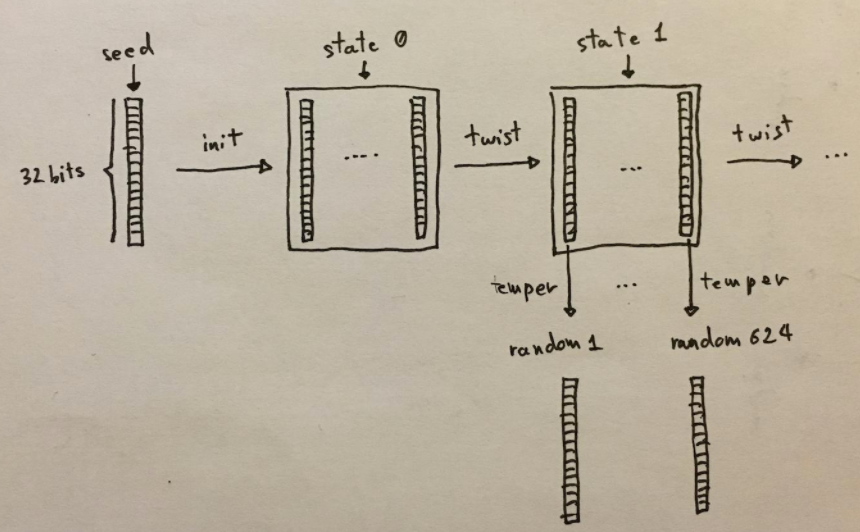
\includegraphics[width = 0.6\textwidth]{figure_man/mersenne.png} \\
\begin{footnotesize}
\url{https://www.cryptologie.net/article/331/how-does-the-mersennes-twister-work/}
\end{footnotesize}
\end{center}


\framebreak

\begin{small}
	\textbf{Note:} Here, random numbers $x_i$ are represented by $w$-bit vectors (usually $w = 32, 64$). To emphasize this, we write $\mathbf{x}_i$ (in bold).
\end{small}

\vspace*{0.2cm}

\textbf{Description of the algorithm:}
\begin{enumerate}
\item \textbf{Initialization: } A seed $\mathbf{x}_0$ is set, and the first $n$ values are calculated based on it (not described here). These values are not part of the final output.
\vspace*{0.2cm}
\begin{center}
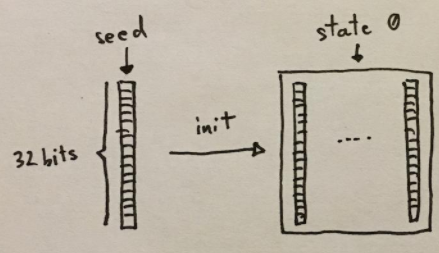
\includegraphics[width = 0.6\textwidth]{figure_man/mersenneinit.png}
\end{center}

\framebreak

\item \textbf{Recursion:} Formally the following recursion formula is used

$$
\mathbf{x}_{k + n} = \mathbf{x}_{k + m}\ \underbrace{\bigoplus}_{3.}\ \underbrace{(\mathbf{x}_{k}^l ||  \mathbf{x}_{k + 1}^r)}_{1.}\ \underbrace{\mathbf{A}}_{2.}
$$

\begin{itemize}
	\item $n$: Degree of recurrence, \enquote{size} of blocks
	\item $m$: Integer $1 \le m < n$
	\item $\mathbf{x}_{k}^l$, $\mathbf{x}_{k}^r$: Left and right part of the vector $x_{k}$
	\item $0 \le c \le w - $1 determines where the \enquote{left part} ends
\end{itemize}

\vspace*{0.2cm}

\begin{center}
	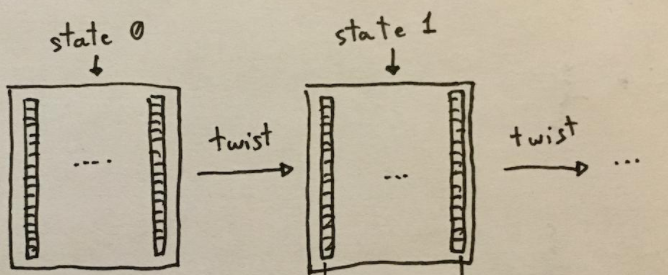
\includegraphics[width = 0.5 \textwidth]{figure_man/twist.png}
\end{center}

\framebreak

For ease of exposition, let $w = 4$, $c = 2$.

\lz

\textbf{1. Concatenation:}

$$
\begin{array}{r} \mathbf{x}_k \\ \mathbf{x}_{k + 1} \\ \mathbf{x}_{k + 2} \end{array}\begin{pmatrix} \textcolor{green}{0} & \textcolor{green}{1} & 1 & 0 \\
\textcolor{red}{1} & \textcolor{red}{0} & \textcolor{green}{1} & \textcolor{green}{0} \\
1 & 1 & \textcolor{red}{1} & \textcolor{red}{1}
\end{pmatrix} \Rightarrow \begin{matrix}
(x_{k}^l || x_{k + 1}^r) & = (\textcolor{green}{0}, \textcolor{green}{1}, \textcolor{green}{1}, \textcolor{green}{0}) \\
(x_{k + 1}^l || x_{k + 2}^r) & = (\textcolor{red}{1}, \textcolor{red}{0}, \textcolor{red}{1}, \textcolor{red}{1})
\end{matrix}
$$

\framebreak
\begin{footnotesize}
\textbf{2. Multiplication by $\mathbf{A}$: }


We multiply with the so-called \textbf{Twist Matrix} $\mathbf{A}$

$$
\mathbf{A} = \begin{pmatrix}
0 & 1 & 0 & 0  \\
0 & 0 & 1 & 0 \\
 0 & 0 & 0 & 1 \\
a_{3} & a_{2} & a_{1} & a_0
\end{pmatrix}
$$

\begin{eqnarray*}
(0, 1, 1, 0)  \mathbf{A} &=& (0, 0, 1, 1)\\
(1, 0, 1, 1) \mathbf{A} &=& (0 \oplus a_3, 1 \oplus + a_2, 0 \oplus a_1, 1 \oplus a_0)
\end{eqnarray*}

In summary $\quad
\mathbf{x}\mathbf{A} = \begin{cases}
\text{shift}(\mathbf{x}), \quad \text{if last bit } x_0 = 0 \\
\text{shift}(\mathbf{x}) \oplus \mathbf{a} , \quad \text{if } x_0 = 1
\end{cases}
$

%\framebreak
\lz

\textbf{3. XOR: }


In the last step a bitwise XOR is calculated, e.g.

$$
\mathbf{x}_{k + m} \bigoplus (0, 0, 1, 1)
$$
\end{footnotesize}

\framebreak

\item \textbf{Tempering:}  In the last step, tempering is applied to the generated random numbers in order to improve their distribution properties.

\vspace*{0.2cm}

\begin{center}
	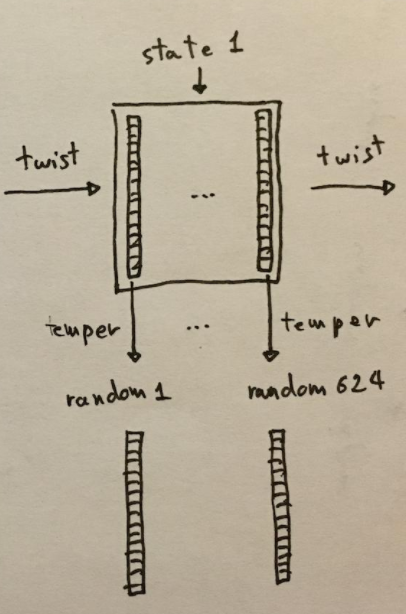
\includegraphics[width = 0.3 \textwidth]{figure_man/temper.png}
\end{center}
\end{enumerate}

\framebreak

The following operations are performed:
\vspace*{-0.2cm}
\begin{eqnarray*}
\mathbf{x} &\mapsto& \mathbf{y} := \mathbf{x} \oplus ((\mathbf{x} >> u) \text{ AND } \mathbf{d}) \\ \mathbf{y} &\mapsto& \mathbf{y} := \mathbf{y} \oplus ((\mathbf{y} << s) \text{ AND } \mathbf{b}) \\
\mathbf{y} &\mapsto& \mathbf{y} := \mathbf{y} \oplus ((\mathbf{y} < < t) \text{ AND } \mathbf{c}) \\ \mathbf{y} &\mapsto& \mathbf{z} := \mathbf{y} \oplus (\mathbf{y} >> l)
\end{eqnarray*}

where $\mathbf{x} >> u$ ($\mathbf{x} << u$) describes the bitwise \enquote{right}-shift (\enquote{left}-shift) by $u$ and \enquote{AND} describes the bitwise \enquote{and}.

\lz

This can be summarized as follows:

$$\mathbf{x} \mapsto \mathbf{z} = \mathbf{x}\mathbf{T}. $$


\framebreak

Coefficients for MT19937: (standard implementation 32-bit)

\begin{description}
  \item[w] word size (in number of bits): 32
  \item[n] degree of recurrence: 624
  \item[m] middle word, an offset used in the recurrence relation defining the series x: 397
  \item[c] separation point of one word, or the number of bits of the lower bitmask: 31
  \item[a] coefficients of the rational normal form twist matrix: $9908B0DF_{16}$
  \item[u, d, l] tempering masks/shifts: $(11, FFFFFFFF_{16}, 18)$
  \item[s, b] tempering masks/shifts: $(7, 9D2C5680_{16})$
  \item[t, c] tempering masks/shifts:  $(15, EFC60000_{16})$
\end{description}

\framebreak


\textbf{Properties}:

\begin{itemize}
	\item Extremely long period of $2^{19937} - 1\approx 4.3 \cdot 10^{6001}$ (so-called \enquote{Mersenne prime})
	\item All bits of the output sequence are uniformly distributed $\to$ thus the corresponding integer values are also uniformly distributed
	\item Low correlation of consecutive values
	\item Fast implementation by calculating $n$ ($n = 624$ in MT19937) random numbers in one step
	\item Highly parallelizable
\end{itemize}

\lz

\footnotesize{
Further information:
\begin{itemize}
	\item \url{www.math.sci.hiroshima-u.ac.jp/~m-mat/MT/ARTICLES/mt.pdf} (Original paper Mersenne Twister)
	\item \url{http://statweb.stanford.edu/~owen/mc/Ch-unifrng.pdf} (Lecture on PRNGs)
\end{itemize}
}
% https://bugs.r-project.org/bugzilla/show_bug.cgi?id=17494

\end{vbframe}


% \subsection{Shift Register Methoden}


% \begin{vbframe}{Twisting / Shuffling}
% Multiplikative und lineare Kongruenzgeneratoren haben zu hohe
% Autokorrelation, insbesondere sind $n$-Tupel nicht gleichverteilt im
% $n$-dimensionalen Einheitswürfel, sondern konzentrieren sich nahe
% weniger Hyperebenen.\\
% \medskip
% Eine einfache Möglichkeit, um zumindest Tupel der Länge $n$ ohne
% Autokorrelation zu bekommen, ist diese automatisch zu mischen.
% \begin{enumerate}
%  \item Initialisiere $s_i=u_i$, $i=1,\ldots,n$, und $y=s_n$.
%  \item Erzeuge neuen Wert $u$, setze $j=\lceil y \cdot n \rceil$.
%  \item Setze $y=s_j$ und $s_j=u$.
%  \item Gib Zufallszahl $y$ zurück, wiederhole ab 2.
% \end{enumerate}
% $u_i$ aus einem Standardgenerator, Seed sind die $n$ Zahlen $s_n$.
%
% \framebreak
%
% <<echo=FALSE>>=
% shuffle = function(n, rand = mkg, ...) {
%   u = mkg(n * 2, ...)
%   s = u[1:n]
%   k = n
%   x = NULL
%   for(i in 1:n) {
%     j = as.integer(s[k] * k) + 1
%     x = c(x, s[k])
%     s[k] = s[j]
%     s[j] = u[n + i - 1]
%   }
%   return(x)
% }
% @
%
% <<echo=FALSE>>=
% randu = shuffle(12000, 1, m = 2^31, a = 2^16 + 3)
% randu3D = as.data.frame(matrix(randu, ncol = 3, byrow = TRUE))
% colnames(randu3D) = c("x1", "x2", "x3")
% @
%
% <<echo=FALSE, rgl=TRUE>>=
% library("rgl")
% mfrow3d(1, 3)
% with(randu3D, plot3d(x1, x2, x3))
% rgl.viewpoint(theta = -12.8, phi = 3.3, fov = 0, zoom = 0.7)
% with(randu3D, plot3d(x1, x2, x3))
% rgl.viewpoint(theta = -6.8, phi = 3.3, fov = 0, zoom = 0.7)
% with(randu3D, plot3d(x1, x2, x3))
% rgl.viewpoint(theta = -3.8, phi = 3.8, fov = 0, zoom = 0.7)
% @
%
% {\footnotesize \emph{Hinweis:} Erneut der selbe Plot
% aus drei verschiedenen Perspektiven.}
%
% % <<>>=
% % z = with(randu, (6 * x2 - 9 * x1) %% 1)
% % head(cbind(z, randu$x3))
% % @
% \end{vbframe}
%
%
% \begin{fragileframe}{Shift-Register-Methode}
% \textbf{Grundlage:} Bei der Shift-Register-Methode wird eine Bitfolge X
% durch Rekursion erzeugt. Für das Element n der Folge gilt:
% $$
% X_n = X_{n-p} \oplus  X_{n-p + q}, \quad 1 < q < p,
% $$
% wobei $\oplus$ für exklusives Oder steht:
%
% \lz
%
% \begin{table}
% \centering
% \begin{tabular}{|cc|c|}
%   \hline
% $X_{n-p}$ & $X_{n-p + q}$  & $X_n$ \\
%   \hline
% \textcolor{green}{0} & \textcolor{green}{0} & \textcolor{red}{0} \\
% \textcolor{green}{0} & \textcolor{green}{1} & \textcolor{red}{1} \\
% \textcolor{green}{1} & \textcolor{green}{0} & \textcolor{red}{1} \\
% \textcolor{green}{1} & \textcolor{green}{1} & \textcolor{red}{0} \\
%    \hline
% \end{tabular}
% \end{table}
%
% Es wird eine Startfolge der Länge p benötigt.
%
%
% <<include=FALSE>>=
% source("rsrc/ieee754.R")
% as.dec.bin("1011")
% as.bin(11)
% as.dec(as.bin(11))
% @
%
% \framebreak
%
% <<echo=FALSE>>=
% shift = function(n, seed = 11, bits = 4, p = 4, q = 3) {
%   x = as.bin(seed, unsigned = TRUE)
%   x = as.integer(strsplit(x, "")[[1]])
%   k = length(x)
%   for(i in 1:(n * bits)) {
%     x = c(x, as.integer(xor(x[k - p + 1], x[k - p + q + 1])))
%     k = length(x)
%   }
%   i = split(1:k, ceiling(seq_along(1:k) / bits))
%   x = as.character(sapply(i, function(j) {
%     paste(x[j], collapse = "")
%   }))
%   x = sapply(x, function(b) {
%     if(nchar(b) < bits) {
%       b = paste(b, paste(rep(0, bits - nchar(b)),
%         collapse = ""),
%       sep = "")
%     }
%     b
%   })
%   ix = sapply(x, as.dec.bin)
%   rval = data.frame(
%     "bin" = x,
%     "int" = ix,
%     "u" = ix / (2^bits),
%     stringsAsFactors = FALSE
%   )
%   rval
% }
% @
%
% % <<eval=FALSE>>=
% % shift = function(n, seed = 11, bits = 4, p = 4, q = 3) {
% %   x = as.bin(seed, unsigned = TRUE)
% %   x = as.integer(strsplit(x, "")[[1]])
% %   k = length(x)
% %   for(i in 1:(n * bits)) {
% %     x = c(x, as.integer(xor(x[k - p + 1], x[k - p + q + 1])))
% %     k = length(x)
% %   }
% %   i = split(1:k, ceiling(seq_along(1:k) / bits))
% %   x = as.character(sapply(i, function(j) {
% %     paste(x[j], collapse = "")
% %   }))
% % @
%
% % <<eval=FALSE>>=
% %   x = sapply(x, function(b) {
% %     if(nchar(b) < bits) {
% %       b = paste(b, paste(rep(0, bits - nchar(b)),
% %         collapse = ""),
% %       sep = "")
% %     }
% %     b
% %   })
% %   ix = sapply(x, as.dec.bin)
% %   rval = data.frame(
% %     "bin" = x,
% %     "int" = ix,
% %     "u" = ix / (2^bits),
% %     stringsAsFactors = FALSE
% %   )
% %   rval
% % }
% % @
%
%
% \textbf{Beispiel:} $p = 4, q = 3$, Startfolge: $1011$.
%
% \begin{footnotesize}
%
% \begin{eqnarray*}
% X_5 &=& X_{1} \oplus  X_{4} = 1 \oplus 1 = 0 \\
% X_6 &=& X_{2} \oplus  X_{5} = 0 \oplus 0 = 0 \\
% X_7 &=& X_{3} \oplus  X_{6} = 1 \oplus 0 = 1 \\
%     &\hdots&
% \end{eqnarray*}
%
% \begin{table}
% \begin{tabular}{rrrrrrrrrr}
%   \hline
%   &   &   & \textcolor{green}{1} & 0 & 1 & 1 & & & \\
%   \hline
% 1 & 0 & 1 & \textcolor{green}{1} & \textcolor{red}{0} & & & & \\
%   \hline
%   \hline
%   &   &   & 1 & \textcolor{green}{0} & 1 & 1 & 0 & &\\
%   \hline
% 1 & 0 & 1 & 1 & \textcolor{green}{0} & \textcolor{red}{0} & & & &\\
%   \hline
%   \hline
%   &   &   & 1 & 0 & \textcolor{green}{1} & 1 & 0 & 0 &\\
%   \hline
% 1 & 0 & 1 & 1 & 0 & \textcolor{green}{0} & \textcolor{red}{1} & & &\\
%   \hline
%   \hline
%   &   &   & 1 & 0 & 1 & \textcolor{green}{1} & 0 & 0 & 1\\
%   \hline
% 1 & 0 & 1 & 1 & 0 & 0 & \textcolor{green}{1} & \textcolor{red}{0} & & \\
%   \hline
% \end{tabular}
% \end{table}
%
% \end{footnotesize}
% \framebreak
%
% <<size="scriptsize">>=
% shift(15)
% @
%
% \framebreak
%
% Im Beispiel codieren Vierergruppen Integer zwischen 1 und 15
% $$
% \text{Zufallszahlen} \quad y_i = \sum\limits_{j=1}^4 2^{-j} X_{4i+j}
% $$
% Periode der Länge $15 = 2^4 - 1$
% (gilt auch für Bits).
% Im Allgemeinen muss nicht gelten, dass Gruppenlänge $M = p$.\\
% \bigskip
% Wahl der Parameter nicht egal. Wähle oben $q = 2$:
%
% <<>>=
% shift(3, q = 2)
% @
%
% \framebreak
%
% Für $q = 1$ und $p = 5$ und Bitlänge 5, erhält man auch nur Periode der Länge 3:
%
% <<>>=
% shift(9, seed = 22, q = 1, p = 5, bits = 5)
% @
% \end{fragileframe}
%
%
% \begin{vbframe}{Generalized Feedback Shift Register (GFSR)}
% Lewis und Payne (1973):
% $$
% y_i = \sum\limits_{j=1}^M 2^{-j} X_{i-s(j)}
% $$
% Typisch: $s(1)=0 < s(2) < \dots < s(M)$ \\
% Ursprünglicher Vorschlag: $s(j) = 100 p (j-1)$, mit $p = 98$ und $q = 27$.
% \begin{itemize}
% \item Liefert große Integer mit langen Perioden $(2^p-1)$.
% \item unabhängig von Maschinenarithmetik (brauche nur $\oplus$)
% \item hervorragende multivariate Eigenschaften
% \end{itemize}
% {\bf Größter Nachteil:}  Nicht triviale Initialisierung. \\
% Benötige Startsequenz der Länge $p$ und nicht jede Startsequenz garantiert optimale Eigenschaften (vgl. Monahan).
% \end{vbframe}
%
%
% \begin{vbframe}{Mersenne-Twister}
% Bei GSFR gilt Rekurrenzrelation für alle Komponenten der Vektoren\\
% $Y_n = [X_n, X_{n - s(2)}, \dots,  X_{n - s(m)}]$.
%
% \lz
%
% {\bf Twisted GFSR}: Variation der Rekursion zu
% $$
% Y_{n+p} = Y_n\ \bigoplus\ (Y_{n+q}^l, Y_{n+q+1}^r)\ \mathbf{A},
% $$
% wobei $Y_{n}^l$ die erste Hälfte und $Y_{n}^r$ die zweite Hälfte
% der Bits und $\mathbf{A}$ eine geeignete Matrix
%
% \lz
%
% {\bf Mersenne-Twister}: Matsumoto und Nishimura (1998),\\
% $p = 624$, $q = 397$, Matrix $\mathbf{A}$ erzeugt nur einfache Bit-Shifts.
% \end{vbframe}


\begin{vbframe}{Transformation to the Interval $(0, 1)$}

\vspace*{-0.4cm}

\begin{itemize}
\item In the procedures discussed, integers between $0$ and $m - 1$ were generated.
\item If real random numbers in the interval $(0, 1)$ need to be simulated, a simple division by $m$ is sufficient.
\item \textbf{Problem:} The random number can be $0$, while for an \enquote{actual} $(0, 1)$ - uniformly distributed random variable $U$ the following holds:
$$
\mathbb{P}(U = 0) = 0
$$
\item This is often a problem in practical applications, e.g. with $\log(U)$.
\item If a $0$ is generated, the random number can be discarded or an error message is issued.
\item Since modern congruential generators have a long period, this is unlikely.
\end{itemize}
%
% \begin{table}
% \begin{footnotesize}
% \centering
% \begin{tabular}{r|rrrrrrrrrr}
%   \hline
%  i & 1 & 2 & 3 & 4 & 5 & 6 & 7 & 8 & 9 & 10 \\
%   \hline
% 0  & 0.29 & 0.94 & 0.41 & 0.12 & 0.18 & 0.76 & 0.65 & 0.47 & 0.71 & 0.06 \\
% 10 & 0.59 & 0.88 & 0.82 & 0.24 & 0.35 & 0.53 & 0.29 & 0.94 & 0.41 & 0.12 \\
% 20 & 0.18 & 0.76 & 0.65 & 0.47 & 0.71 & 0.06 & 0.59 & 0.88 & 0.82 & 0.24 \\
% 30 & 0.35 & 0.53 & 0.29 & 0.94 & 0.41 & 0.12 & 0.18 & 0.76 & 0.65 & \ldots \\
%    \hline
% \end{tabular}
% \end{footnotesize}
% \end{table}

\end{vbframe}

\begin{vbframe}{PRNGs in R}
The Mersenne Twister is (currently) the default method in R with period
$2^{19937} - 1 \approx 10^{6001}$ and guaranteed uniform distribution in
623 dimensions.
Seeds are 624 32-bit integers on top of the current position in this set. The \code{set.seed()} function generates a valid seed from a
single integer value using the linear congruential generator with
$$
  m=2^{32}, \qquad a=69069, \qquad b=1
$$
There are a number of other generators available. Furthermore, the
user can also specify her own generator as default.
\code{RNGversion('x.y.z')} can be used to set the random generators as they were in an earlier R version (for reproducibility) (Wichman-Hill up to 0.98, Marsaglia-Multicarry up to 0.00).
1.6.1). Initialization of the seed via time.
\end{vbframe}


\begin{vbframe}{R: Random Number Generation}
\begin{itemize}
%\begin{footnotesize}
\item \code{set.seed()} function

\footnotesize
\begin{verbbox}
set.seed(123); u1 <- runif(100)
set.seed(123); u2 <- runif(100) 
identical(u1, u2) # the same because of identical RNG status
## [1] TRUE
\end{verbbox}
\col

\normalsize
\item \code{.Random.seed()} is an integer vector, containing the random number generator (RNG) state for random number generation in R. It can be saved and restored, but should not be altered by the user.

\item \code{RNGkind()} is a more friendly interface to query or set the kind of RNG in use.
\footnotesize

\begin{verbbox}
# default for "kind", "normal kind" and "sample kind" 
RNGkind("default") 
RNGkind()
## [1] "Mersenne-Twister" "Inversion"  "Rejection"
.Random.seed[1:3] # the default random seed is 626 integers
## [1] 10403 624 1858651209
\end{verbbox}
\col

\normalsize
\framebreak
\item Change default of kind ("Mersenne-Twister") to "Wichmann-Hill"

\footnotesize
\begin{verbbox}
RNGkind("Wich")
RNGkind()
## [1] "Wichmann-Hill" "Inversion" "Rejection"
.Random.seed
## [1] 10400  5989  8337  9843
\end{verbbox}
\col

\normalsize
\item Change methods depending on defaults in a specific R Version

\footnotesize
\begin{verbbox}
RNGversion(getRversion()) # current version
RNGkind()
## [1] "Mersenne-Twister" "Inversion" "Rejection"
RNGversion("1.0.0") # first R version
## Warning in RNGkind("Marsaglia-Multicarry", "Buggy
Kinderman-Ramage", "Rounding"): buggy version of 
Kinderman-Ramage generator used
## Warning in RNGkind("Marsaglia-Multicarry", "Buggy
Kinderman-Ramage", "Rounding"): non-uniform 'Rounding' 
sampler used
\end{verbbox}
\col

%\end{footnotesize}
\end{itemize}
\end{vbframe}





\begin{vbframe}{Parallel computing}
A complex topic is the application of random number generators for parallel computing, where a long calculation is split between several machines and processed in parallel.
Usually, a \enquote{master} distributes the jobs to several \enquote{slaves}.
Initialization of seed using the two \enquote{standard} methods
\begin{itemize}
  \item Time of day or
  \item Fixed given number
\end{itemize}
is not useful.
Special algorithms for this purpose are provided e.g. in the R packages \texttt{rlecuyer} or
\texttt{rstreams} (both use the same algorithm from L'Ecuyer).
\end{vbframe}



\endlecture


\end{document}